\documentclass[12pt,a4paper, spanish]{report}
\usepackage[spanish]{babel}
\usepackage[latin1]{inputenc}  % Ambos para solucin de asuntos de idioma
\usepackage[T1]{fontenc}
\usepackage{tocbibind}  % Bibliografa en el indice
\usepackage{titlesec}  % Posibilidad de editar los formatos de chapter y section
%\usepackage{times}  % Fuente de letras
\usepackage{amsmath,amssymb,mathrsfs,mathptmx}  % Matemticas varias
\usepackage{hyperref} % Para escribir URLs



% --- Arreglos varios para la inclusion de imgenes
%\usepackage[pdftex]{graphicx}
%\usepackage[dvips]{graphicx}
\usepackage{graphicx}
%\usepackage{epstopdf}
\usepackage{epstopdf}
\usepackage{float}
\usepackage{subfigure}
%\usepackage{subfig}
\usepackage{wrapfig}
\usepackage[usenames,dvipsnames]{color}
\DeclareGraphicsExtensions{.png,.jpg,.pdf,.mps,.gif,.bmp, .eps}




\usepackage{multirow}
\usepackage{multicol}
\usepackage{tabulary}
\usepackage[table]{xcolor}
\usepackage{color}
\usepackage{listings}
%\usepackage{subfloat}
\usepackage{tikz}

\setcounter{secnumdepth}{3}
\setcounter{tocdepth}{3}


% --- Para las dimensiones de los mrgenes etc
\frenchspacing \addtolength{\hoffset}{-1.5cm}
\addtolength{\textwidth}{3cm} \addtolength{\voffset}{-2.5cm}
\addtolength{\textheight}{4cm}
% --- Para el encabezado
\usepackage{fancyhdr}
\fancyhead[R]{2012}\fancyhead[L]{enCuadro} \fancyfoot[C]{\thepage}
\pagestyle{fancy}

% --- Formato de la etiqueta Chapter
%\newcommand{\bigrule}{\titlerule[0.5mm]}
%\titleformat{\chapter}[display]{\bfseries\Huge}
%{\Large\chaptertitlename\ \Large\thechapter}
%{0mm} {\filleft} [\vspace{0.5mm} \bigrule]

\titleformat{\chapter}[display]
{\normalfont\Large\filcenter}
{\titlerule[1pt]%
\vspace{1pt}%
\titlerule
\vspace{1pc}%
\LARGE\MakeUppercase{\chaptertitlename} \thechapter}
{1pc}
{\titlerule
\vspace{1pc}%
\Huge}

%-------------------------

\begin{document}
% Esto es para que se muestren todas las referencias aunque no se citen:
\nocite{*}

\renewcommand{\tablename}{Tabla}
\renewcommand{\theenumi}{\Roman{enumi}}
\renewcommand{\labelenumi}{[\textbf{\theenumi}]}
\renewcommand{\thefootnote}{\arabic{footnote}}
% --- Modificacin de entornos enumerate
\renewcommand{\theenumi}{\roman{enumi}}
\renewcommand{\labelenumi}{\theenumi)}
% --- Modificacin de entornos enumerate

% --- Para hacer highlights
\newcommand{\highlAmarillo}[1]{\colorbox{yellow}{#1}}
\newcommand{\highlVerde}[1]{\colorbox{green}{#1}}
\newcommand{\highlRojo}[1]{\colorbox{red}{#1}}

%



\chapter{LSD: ``Line Segment Detection''}

\section{Introducci�n}
LSD es un algoritmo de detecci�n de segmentos publicado por Rafael Grompone von Gioi, J�r�mie Jakubowicz, Jean-Michel Morel y Gregory Randall en abril de 2010. Es temporalmente lineal, tiene presici�n inferior a un p�xel y no requiere de un tuneo previo de par�metros, como casi todos los dem�s algoritmos de id�ntica funci�n; puede ser considerado el estado del arte en cuanto a detecci�n de segmentos en im�genes digitales. Como cualquier otro algoritmo de detecci�n de segmentos, LSD basa su estudio en la b�squeda de contornos angostos dentro de la imagen. Estos son regiones en donde el nivel de brillo de la imagen cambia notoriamente entre p�xeles vecinos, por lo que el gradiente de la misma resulta de vital importancia. Se genera previo al an�lisis de la imagen, un campo de orientaciones asociadas a cada uno de los p�xeles denominado por los autores \textit{level-line orientation field}. Dicho campo se obtiene de calcular las orientaciones ortogonales a los �ngulos asociados al gradiente del la imagen. Luego, LSD puede verse como una composici�n de tres pasos:\\
\begin{itemize}
\item[(1)] Divisi�n de la imagen en las llamadas \textit{line-support regions}, que son grupos conexos de p�xeles con id�ntica orientaci�n, hasta cierta tolerancia. 
\item[(2)] B�squeda del segmento que mejor aproxime cada  \textit{line-support region}: aproximaci�n de las regiones por rect�ngulos.
\item[(3)] Validaci�n o no de cada segmento detectado en el punto anterior. 
\end{itemize}
Los puntos (1) y (2) est�n basados en el algoritmo de detecci�n de segmentos de Burns, Hanson y Riseman y el punto (3) es una adaptaci�n del m�todo \textit{a contrario} de Desolneux, Moisan y Morel. 

\section{\textit{Line-support regions}}
El primer paso de LSD es el dividir la imagen en regiones conexas de p�xeles con igual orientaci�n, a menos de cierta tolerancia $\tau$, llamadas \textit{line-support regions}. El m�todo para realizar tal divisi�n es del tipo ``regi�n creciente''; cada regi�n comienza por un p�xel y cierto �ngulo asociado al mismo. Luego, se testean sus ocho vecinos y los que cuenten con un �ngulo similar al del p�xel original son inclu�dos en la regi�n. En cada iteraci�n el �ngulo asociado a la regi�n es calculado como el promedio de las orientaciones de cada p�xel dentro de la \textit{line-support region}; la iteraci�n termina cuando ya no se pueden agregar m�s p�xeles a la misma.\\

\begin{figure}[h!]
\centering
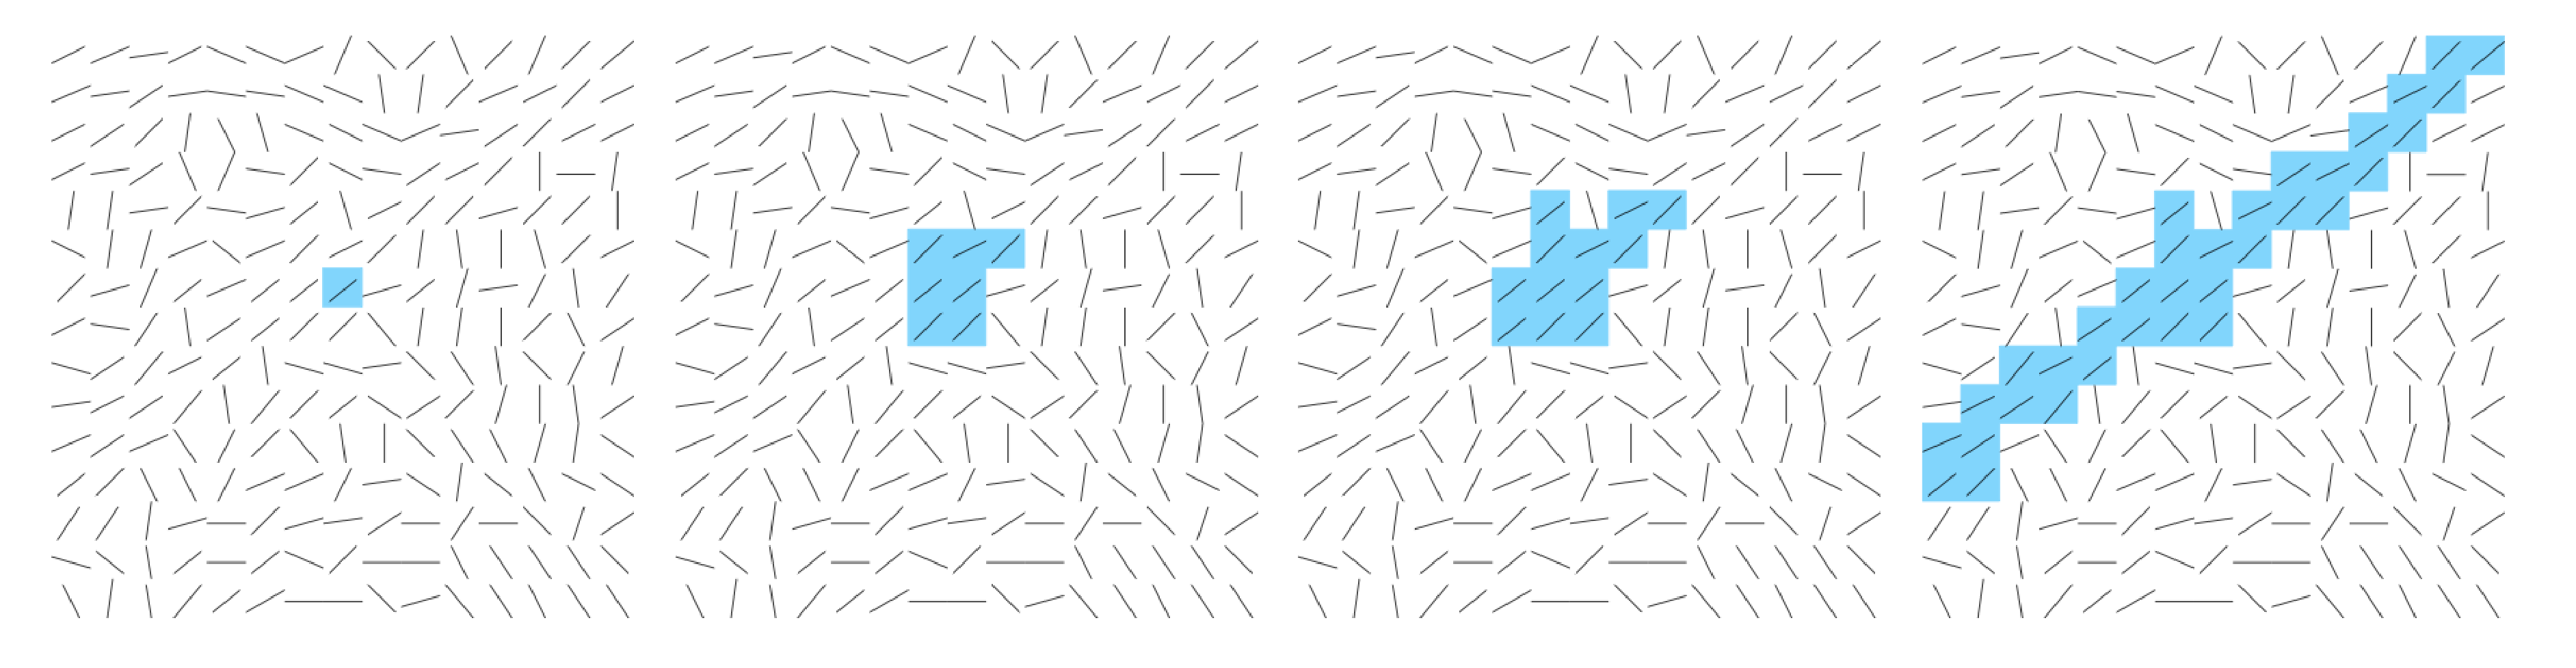
\includegraphics[scale=0.2]{figs_lsd/lsd_1.eps}
\caption{Proceso de crecimiento de una regi�n. El �ngulo asociado cada p�xel de la imagen est� representado por los peque\~nos segmentos y los p�xeles coloreados representan la formaci�n de la regi�n. Fuente \cite{grompone10}.}
\label{fig: lsd_1}
\end{figure}

Los p�xels agregados a una regi�n son marcados de manera que no se vuelvan a testear. Para mejorar el desempe\~no del algoritmo, las regiones comienzan a evaluarse por los p�xeles con gradientes de mayor amplitud ya que estos representan mejor los bordes. \\
Existen algunos casos puntuales en los que el proceso de b�squeda de \textit{line-support regions} puede arrojar errores. Por ejemplo, cuando se tienen dos segmentos que se juntan y que son colineales a no ser por la tolerancia $\tau$ descripta anteriormente, se detectar�n ambos segmentos como uno solo; ver figura \ref{fig: lsd_2}. Este potencial problema es heredado del algoritmo de Burns, Hanson y Riseman.

\begin{figure}[h!]
\centering

\includegraphics[scale=0.25]{figs_lsd/lsd_2.eps}
\caption{Potencial problema heredado del algoritmo de Burns, Hanson y Riseman. Izq.: Imagen original. Ctro.: Segmento detectado. Der.: Segmentos que deber�an haberse detectado. Fuente \cite{grompone10}.}
\label{fig: lsd_2}
\end{figure}

Sin embargo, LSD plantea un m�todo para ahorraste este tipo de problemas. Durante el proceso de crecimiento de las regiones, tambi�n se realiza la aproximaci�n rectangular a dicha regi�n (paso (2) de los tres definidos anteriormente); y si menos del $50\%$ de los p�xeles dentro del rect�ngulo corresponden a la \textit{line-support region}, entonces lo que se tiene no es un segmento. Se detiene entonces el crecimiento de la regi�n.

\section{Aproximaci�n de las regiones por rect�ngulos}

\begin{figure}[h!]
\centering
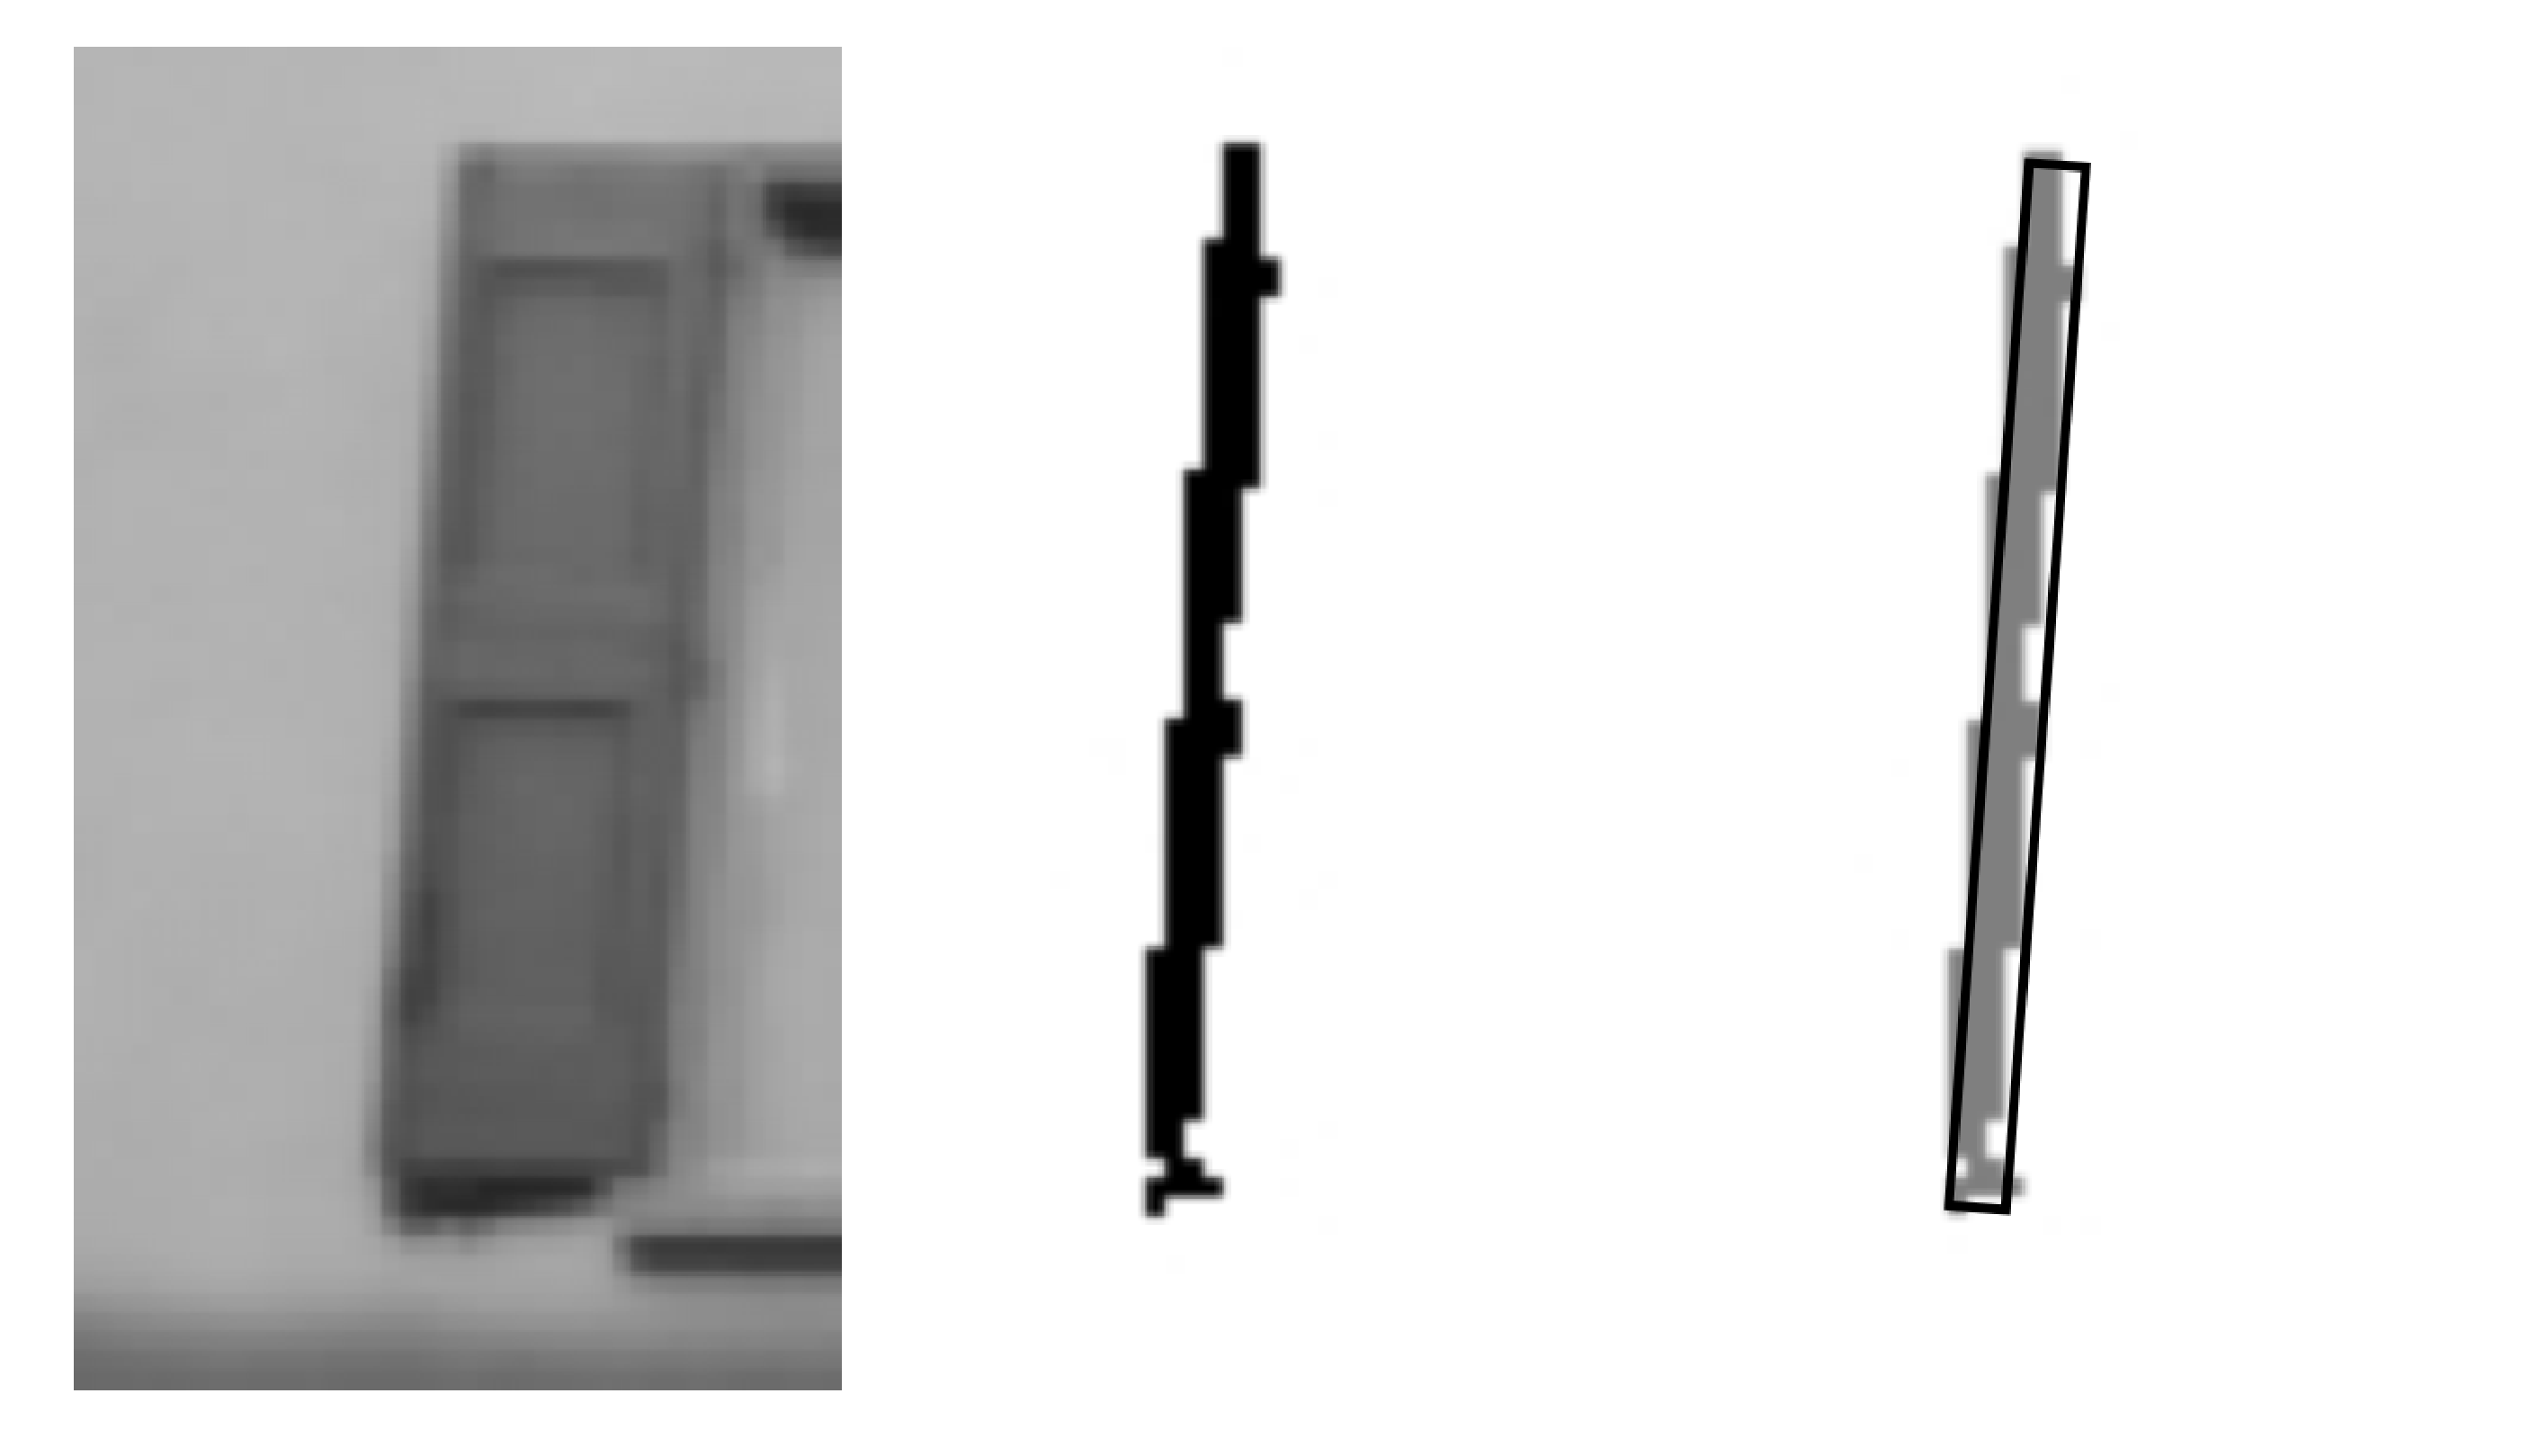
\includegraphics[scale=0.2]{figs_lsd/lsd_3.eps}
\caption{B�squeda del segmento que mejor aproxime cada \textit{line-support region}: aproximaci�n de una regi�n por un rect�ngulo. Izq.: Imagen original. Ctro.: Una de las regiones computadas. Der.: Aproximaci�n rectangular que cubre el $99\%$ de la masa de la regi�n. Fuente \cite{grompone10}.}
\label{fig: lsd_3}
\end{figure}

Cada \textit{line-support region} debe ser asociada a un segmento. Cada segmento ser� determinado por su centro, su direcci�n, su anchura y su longitud. A diferencia de lo que pudi�se dictar la intuici�n, la direcci�n asociada al segmento no se corresponde con la asociada a la regi�n (el promedio de las direcciones de cada uno de los p�xeles). Sin embargo, se elige el centro del segmento como el centro de masa de la regi�n y su direcci�n como el eje de inercia principal de la misma; la magnitud del gradiente asociado a cada p�xel hace las veces de masa. La idea detr�s de este m�todo es que los p�xeles con un gradiente mayor en m�dulo, se corresponden mejor con la percepci�n de un borde. La anchura y la longitud del segmento son elegidos de manera de cubir el $99\%$ de la masa de la regi�n.

\section{Validaci�n de segmentos}
La validaci�n de los segmentos previamente detectados se plantea como un m�todo de test de hip�tesis. Se utiliza un modelo \textit{a-contrario}: dada una imagen, sin ning�n tipo de estructura, de ruido blanco y Gaussiano; se sabe que cualquier detecci�n sobre la misma ser� casual y por lo tanto irrelevante. En rigor, se sabe que para cualquier imagen de este tipo, su \textit{level-line oriantation field} toma, para cada p�xel, valores independientes y uniformemente distribu�dos entre $[0,2\pi]$. Dado entonces un segmento en la imagen analizada, se estudia la posibilidad de que dicha detecci�n se d� en la imagen de ruido, y si la probabilidad es lo suficientemente baja, se la considerar� una detecci�n v�lida, de lo contrario se considerar� que se esta bajo la hip�tesis $H_0$: un conjunto aleatorio de p�xeles que casualmente se alinearon de manera de detectar un segmento.\\
Para estudiar la probabilidad de una cierta detecci�n en la imagen de ruido, se deben tomar en cuenta todos los posibles rect�ngulos en la imagen. Dada una imagen $N\times N$, habr�n $N^4$ orientaciones potenciales para los segmentos, $N^2$ puntos de inicio y $N^2$ puntos de fin. Si se consideran $N$ posibles valores para la anchura de los rect�ngulos, se obtienen $N^5$ posibles segmentos. Por su parte, dado cierto rect�ngulo $r$, detectado en la imagen $x$, se denota $k(r,x)$ a la cantidad de p�xeles alineados dentro del mismo. Se define adem�s un valor llamado \textit{Number of False Alarms} (NFA) que corresponde a la probabilidad de detectar al rect�ngulo en cuesti�n en la imagen de ruido $X$:
\[
NFA(r,x) = N^5\P_{H_0}
\]


% Ejemplo de como hacer una cita:
%\cite{Daniel03simultaneouspose}.



\bibliographystyle{unsrt}   
\bibliography{encuadro}  
\end{document}
